\documentclass[a4paper]{article}
% Packages
\usepackage{amsmath} % For math symbols and equations
\usepackage{amssymb} % For math symbols
\usepackage{enumerate} % For custom numbering of lists
\usepackage{cancel} % for extra in math
\usepackage[
  inner=2cm, % Set inner margin to 2 cm
  outer=2cm, % Set outer margin to 2 cm
  bindingoffset=0.5cm, % Set binding offset to 0.5 cm
  top=2cm, % Set top margin to 2 cm
  bottom=2cm % Set bottom margin to 2 cm
]{geometry}
\usepackage{fancyhdr} % For custom headers and footers
\usepackage{lastpage} % For referencing the last page number
\usepackage{titlesec} % For custom section and subsection headings
\usepackage[version=4]{mhchem} % Required package for chemical equations
\usepackage{hyperref} % connections
\usepackage{parskip} % skip paragraphs
\usepackage[
backend=biber,
sorting=anyvt,
style = ieee
]{biblatex} % for using references
\usepackage{setspace}
\usepackage{graphicx}
\usepackage{caption}
\usepackage{adjustbox}
\usepackage{booktabs}
\usepackage{enumitem}
\usepackage{tikz}
\usepackage{multicol}
\addbibresource{hw2refs.bib}

% Page setup
\pagestyle{fancy} % Set page style to fancy
\fancyhf{} % Clear default headers and footers
\lhead{Bekir Şahin} % Set left header to your name
\rhead{ENVE422 - Homework 2} % Set right header to assignment name
\cfoot{\thepage\ / \pageref{LastPage}} % Set footer to page number

% custom enumeration
\newlist{sludgenum}{enumerate}{1}
\setlist[sludgenum]{label={\textbf{Sludge \arabic*:}}, align=left, wide = 0pt}

% Section and subsection setup
\titleformat{\section}{\large\bfseries}{Question \thesection}{1em}{} % Set section format
\titleformat{\subsection}{\bfseries}{Part \thesubsection}{1em}{} % Set subsection format
\titlespacing{\section}{0pt}{0.25\baselineskip}{0.25\baselineskip} % Adjust spacing before and after section
\titlespacing{\subsection}{0pt}{0.25\baselineskip}{0.25\baselineskip} % Adjust spacing before and after subsection

% Document information
\title{Department of Environmental Engineering\\Middle East Technical University\\Spring 2023\\ENVE422\\Treatment and Disposal of Water \& Wastewater Sludges\\Homework 2 Submission} % Set document title
\author{\href{sahin.bekir@metu.edu.tr}{Bekir Şahin}} % Set document author
\begin{document}
\setcounter{page}{0}
\onehalfspacing
\maketitle % Add title to document
\thispagestyle{empty}
\newpage
\section{}
A mass balance for completely mixed continuous aerobic digester \autocite{metcalf2014} can be written as:
\begin{equation}
    \text{Input} - \text{Output} - \text{Change in reactor} = \text{Net Change} \label{eq:massbalance}
\end{equation}
\begin{minipage}[c]{0.5\textwidth}
Using the Equation \ref{eq:massbalance}, the following mass balance can be written for the VSS content:
$$\frac{dS}{dt}*V = Q_{in} S_{in} - Q_{out} S + V r$$
$$r = -K_dS$$
All sides are divided by the volume:
$$\cancelto{\text{0 since SS}}{\frac{dS}{dt}} = \frac{Q_{in} S_{in}}{V} - \frac{Q_{out} S}{V} - K_dS$$
Since there is no change in flow, both can be notated by $Q$:
$$0 = \frac{Q S_{in}}{V} - \frac{Q S}{V} - K_d S$$
\end{minipage}
\hfill
\begin{minipage}{0.4\textwidth}
\fbox{\parbox{0.95\textwidth}{\textbf{Assumptions}\\Aerobic digestion\\Completely mixed, continuous flow\\Steady state\\Fixed volume ($V$)\\$Q_{in} = Q_{out}$\\$K_d = 0.1 \text{ day}^{-1}$}}
\end{minipage}
\begin{equation}
    V = \frac{Q (S_{in} -  S)}{K_d S } \label{eq:volume}
\end{equation}
We can calculate the desired effluent concentration by knowing the daily flow and loading rates. With 50\% VSS reduction, the effluent concentration is $\mathbf{41\frac{2}{3}}$ kg/m$^3$. Using the Equation \ref{eq:volume}, the volume for the digester can be calculated as follows:
$$V=\frac{500\text{ kg/d}-250\text{ kg/d}}{0.1\text{/d}*41\frac{2}{3}\text{ kg/m}^3}=\boxed{60 \text{ m}^3}$$
\section{}
\section*{Theory}
Composting can be divided into 2 crucial stages \autocite{Eliot1997, metcalf2014}. In the first, high-rate composting stage, the thermophilic organisms are favored, and the high temperature takes on for almost 30 days \autocite{vesilind1988}. In the second stage, curing starts, the compost starts to cool off, and microbial activity decreases as time goes on \autocite{vesilind1988, metcalf2014}.\\
During the first stage, the aeration is supplied, and during this period, sludge is stabilized with high rates \autocite{sanin2011}. In the curing state, compost is let to sit to stabilize itself further while waiting to be marketed.\\
In this method, \textsl{static pile air vessel} system, the sludge is not agitated by any mechanics. In our case, a bulking agent, woodchips, gives easy access to air to move by forming passages and drop moisture content \autocite{sanin2011, vesilind1988}.\\
Some of the parameters that are essential while operating the composting \textbf{C/N} ratio, \textbf{moisture \%} \autocite{sanin2011, metcalf2014, vesilind1988}. Moreover, some other parameters should be considered such as \textbf{availability of minerals}, \textbf{pH}, \textbf{oxygen availability} \autocite{sanin2011}.\\
C/N ratio is not an issue for sludge in most cases \autocite{vesilind1988}. It is possible to operate with C/N ratio with 20:1. Moisture should be higher than 40\% but not higher than 60\% since it creates anaerobic clumps \autocite{vesilind1988}.\\
Woodchips are good bulking agents in these systems due to their high recovery rate and carbon supplemental properties \autocite{metcalf2014}.
\section*{Design Procedure}
One of the parameters that should be determined for designing such a system is the residence time of compost in high-rate composting and curing stages. Finding a sensible \textbf{retention time} while considering the stability of sludge depends on many parameters such as climate, aeration availability, etc. \autocite{sanin2011}. According to \textcite{vesilind1988} and the studies they had shown, the high-rate composting stage ends near 30 days and compost starts to cure. Although most of the pathogenic microbial activity slows down in this stage, there are persistent ones as shown by \textcite{sanin2011}. I will assume composting and curing duration as \textbf{90 days}. After \textsl{30 days of high rate composting}, \textsl{60 days for curing stage} will be enough time for compost to restabilize itself regarding microbial activity while not overestimating the time requirement.\\
Another consideration is the system configuration and the shape of the windrows that are put together. The height is assumed to be 1.8 m, while the width should be in a range where the aeration can be achieved efficiently, and the configuration must be kept in mind. Since we are talking about windrows, I assumed it would be in a triangle shape (as in Figure \ref{fig:windrow}) because the heavy machinery puts the compost on top of the system.\\
Some guidelines for details on the total area composition are illustrated in Equation \ref{eq:total_area}. Furthermore, all the given and asked parameters are given in the following section.
\begin{multicols}{2}
\section*{Given}
\begin{itemize}
    \item 120 metric tons daily intake = 120000 kg/d
    \item Solids content 30\% (not affecting the area calculation since there is no material balance)
    \item $\rho = 1009\text{ kg/m}^3$
    \item 60\% of the total area is for runoff collection
    \item Volumetric ratio of 3:1 with woodchips
\end{itemize}
\columnbreak
\section*{Determined}
\begin{itemize}
    \item Baseline width = 2.5 - 4.0 m \autocite{sanin2011, metcalf2014, vesilind1988}
    \item Composting time (based on many parameters) = 21 - 28 d \autocite{metcalf2014}
    \item Curing duration (depends on the goals of the process) = 30+ d \autocite{metcalf2014}
    \item Finding the area required for the windrows using Figure \ref{fig:windrow}
    \item Total Area using Equation \ref{eq:total_area}
\end{itemize}
\end{multicols}
\begin{figure}[ht]
    \centering
    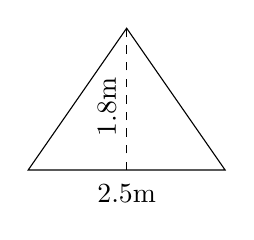
\begin{tikzpicture}
        \draw (0,0) -- (2.5,0) -- (1.25,1.8) -- cycle;
        \draw[dashed] (1.25,0) -- (1.25,1.8);
        \node at (1.0, 0.8) [rotate=90]  {1.8m};
        \node at (1.25, -0.3) {2.5m};
    \end{tikzpicture}
    \caption{Dimensions for the windrows}
    \label{fig:windrow}
\end{figure}
\begin{equation}
    \text{{0.4A}} :
\begin{bmatrix}
    \text{composting + curing} \\
    =\\
    \text{composting + curing + roads + turnarounds} \\
\end{bmatrix}
+
\text{{0.6A}} :
\begin{bmatrix}
    \text{runoff collection}
\end{bmatrix}
=
\text{Total Area (A)}
\label{eq:total_area}
\end{equation}
\section*{Calculations}
\textbf{Daily volumetric sludge intake:}
$$\frac{120*10^3 \text{ kg/d}}{1009 \text{ kg/m}^3} = 118.93 \text{ m}^3\text{/d}$$
\textbf{Amendment with a bulking agent (3 to 1 ratio):}
$$118.93 \text{ m}^3\text{/d} * 4 = 475. 72 \text{ m}^3\text{/d}$$
\textbf{Retention time of 90 days for composting and curing requires:}
$$475. 72 \text{ m}^3\text{/d} * 90 \text{ days} = 42814.67 \text{ m}^3 \text{ in the facility.}$$
\textbf{The area required (\boldmath{$2.5L$}):}
$$\frac{2.5L\text{ m}^2*1.8\text{ m}}{2}=42814.67 \text{ m}^3 $$
$$\text{Composting + Curing Area : } \frac{2*42814.67\text{ m}^3}{1.8\text{ m}}=47571.85 \text{ m}^2$$
$$\text{Runoff Collection Area : } \frac{0.6*47571.85}{0.4}=71357.78 \text{ m}^2$$
$$\text{Total Area : } 118929.63 \text{ m}^2 \approx 118930 \text{ m}^2 \approx \textbf{12 ha}$$
\section{}
The given shear stress (Pa) and shear rate (1/s) are tabulated in Table \ref{tab:rheology} and scatter plot with different shapes in Figure \ref{fig:SludgeShear}.
\begin{table}[ht]
    \caption{Shear stress (N/m$^2$) and shear rate (1/s) values for Sludge 1, Sludge 2, and Sludge 3}
    \centering
    \begin{tabular}{cccccc}
         \toprule
         \multicolumn{2}{c}{\textbf{Sludge 1}} & \multicolumn{2}{c}{\textbf{Sludge 2}} & \multicolumn{2}{c}{\textbf{Sludge 3}} \\
         \cmidrule(lr){1-2} \cmidrule(lr){3-4} \cmidrule(lr){5-6}
         Shear Stress & Shear Rate & Shear Stress & Shear Rate & Shear Stress & Shear Rate \\
         N/m$^2$ & s$^{-1}$ & N/m$^2$ & s$^{-1}$ & N/m$^2$ & s$^{-1}$ \\
         \cmidrule(lr){1-1} \cmidrule(lr){2-2} \cmidrule(lr){3-3} \cmidrule(lr){4-4} \cmidrule(lr){5-5} \cmidrule(lr){6-6}
         3.8	& 1.8	& 1.7	& 1.8	& 15.4	& 1.8 \\
         5.4	& 3.7	& 3.6	& 3.7	& 17.3	& 3.7 \\
         9.0	& 7.3	& 7.5	& 7.3	& 21.3	& 7.3 \\
         14.1 & 14.7	& 15.0	& 14.7 & 28.7 & 14.7 \\
         23.1 & 36.7 & 36.9 & 36.7 & 50.6 & 36.7 \\
         35.7 & 73.4 & 74.2 & 73.4 & 87.9 & 73.4 \\
         \bottomrule
    \end{tabular}
    \label{tab:rheology}
\end{table}
\begin{sludgenum}
    \item \textsl{Shear thinning} behavior can be expressed as curves starting from the origin and concave upwards as shear rate increases; that is, shear rate increases less proportional to shear stress \autocite{Rao2014}. These types of fluids are called \textit{pseudoplastic} fluids. The shear breaks down the structures in the fluid, making it a thinner complex \autocite{sanin2011, dick1967}.\\
    Performing a power series regression for Sludge 1 values results in 0.95 as the intercept and 0.61 as the slope with 0.9977 $R^2$ value. Thus, Sludge 1 is categorized as \textbf{pseudoplastic fluid}.
    \item For the case of \textsl{Newtonian} fluids, the shear rate is directly proportional to shear stress, and the plotting begins from the origin \autocite{Rao2014}.\\
    If the Sludge 2 values are checked, it can be seen that this is the case. Linear regression for that sludge shear rates and shear stresses yields intercept as -0.03 and the slope as 1.01 with $R^2$ equaling 1. Since the intercept value is close to 0, the intercept can be regarded as 0. Therefore, Sludge 2 shows \textbf{Newtonian} characteristics.
    \item In cases where the flow does not start until a threshold shear stress value, followed by a straight line follows \textsl{Bingham plastic} model \autocite{Rao2014}.\\
    The linear model conducted for Sludge 3 gives the intercept as 13.70 and the slope as 1.01 with a $R^2$ value of 1. As a result, Sludge 3 follows \textbf{Bingham plastic} model.
\end{sludgenum}
\begin{figure}[ht]
    \centering
    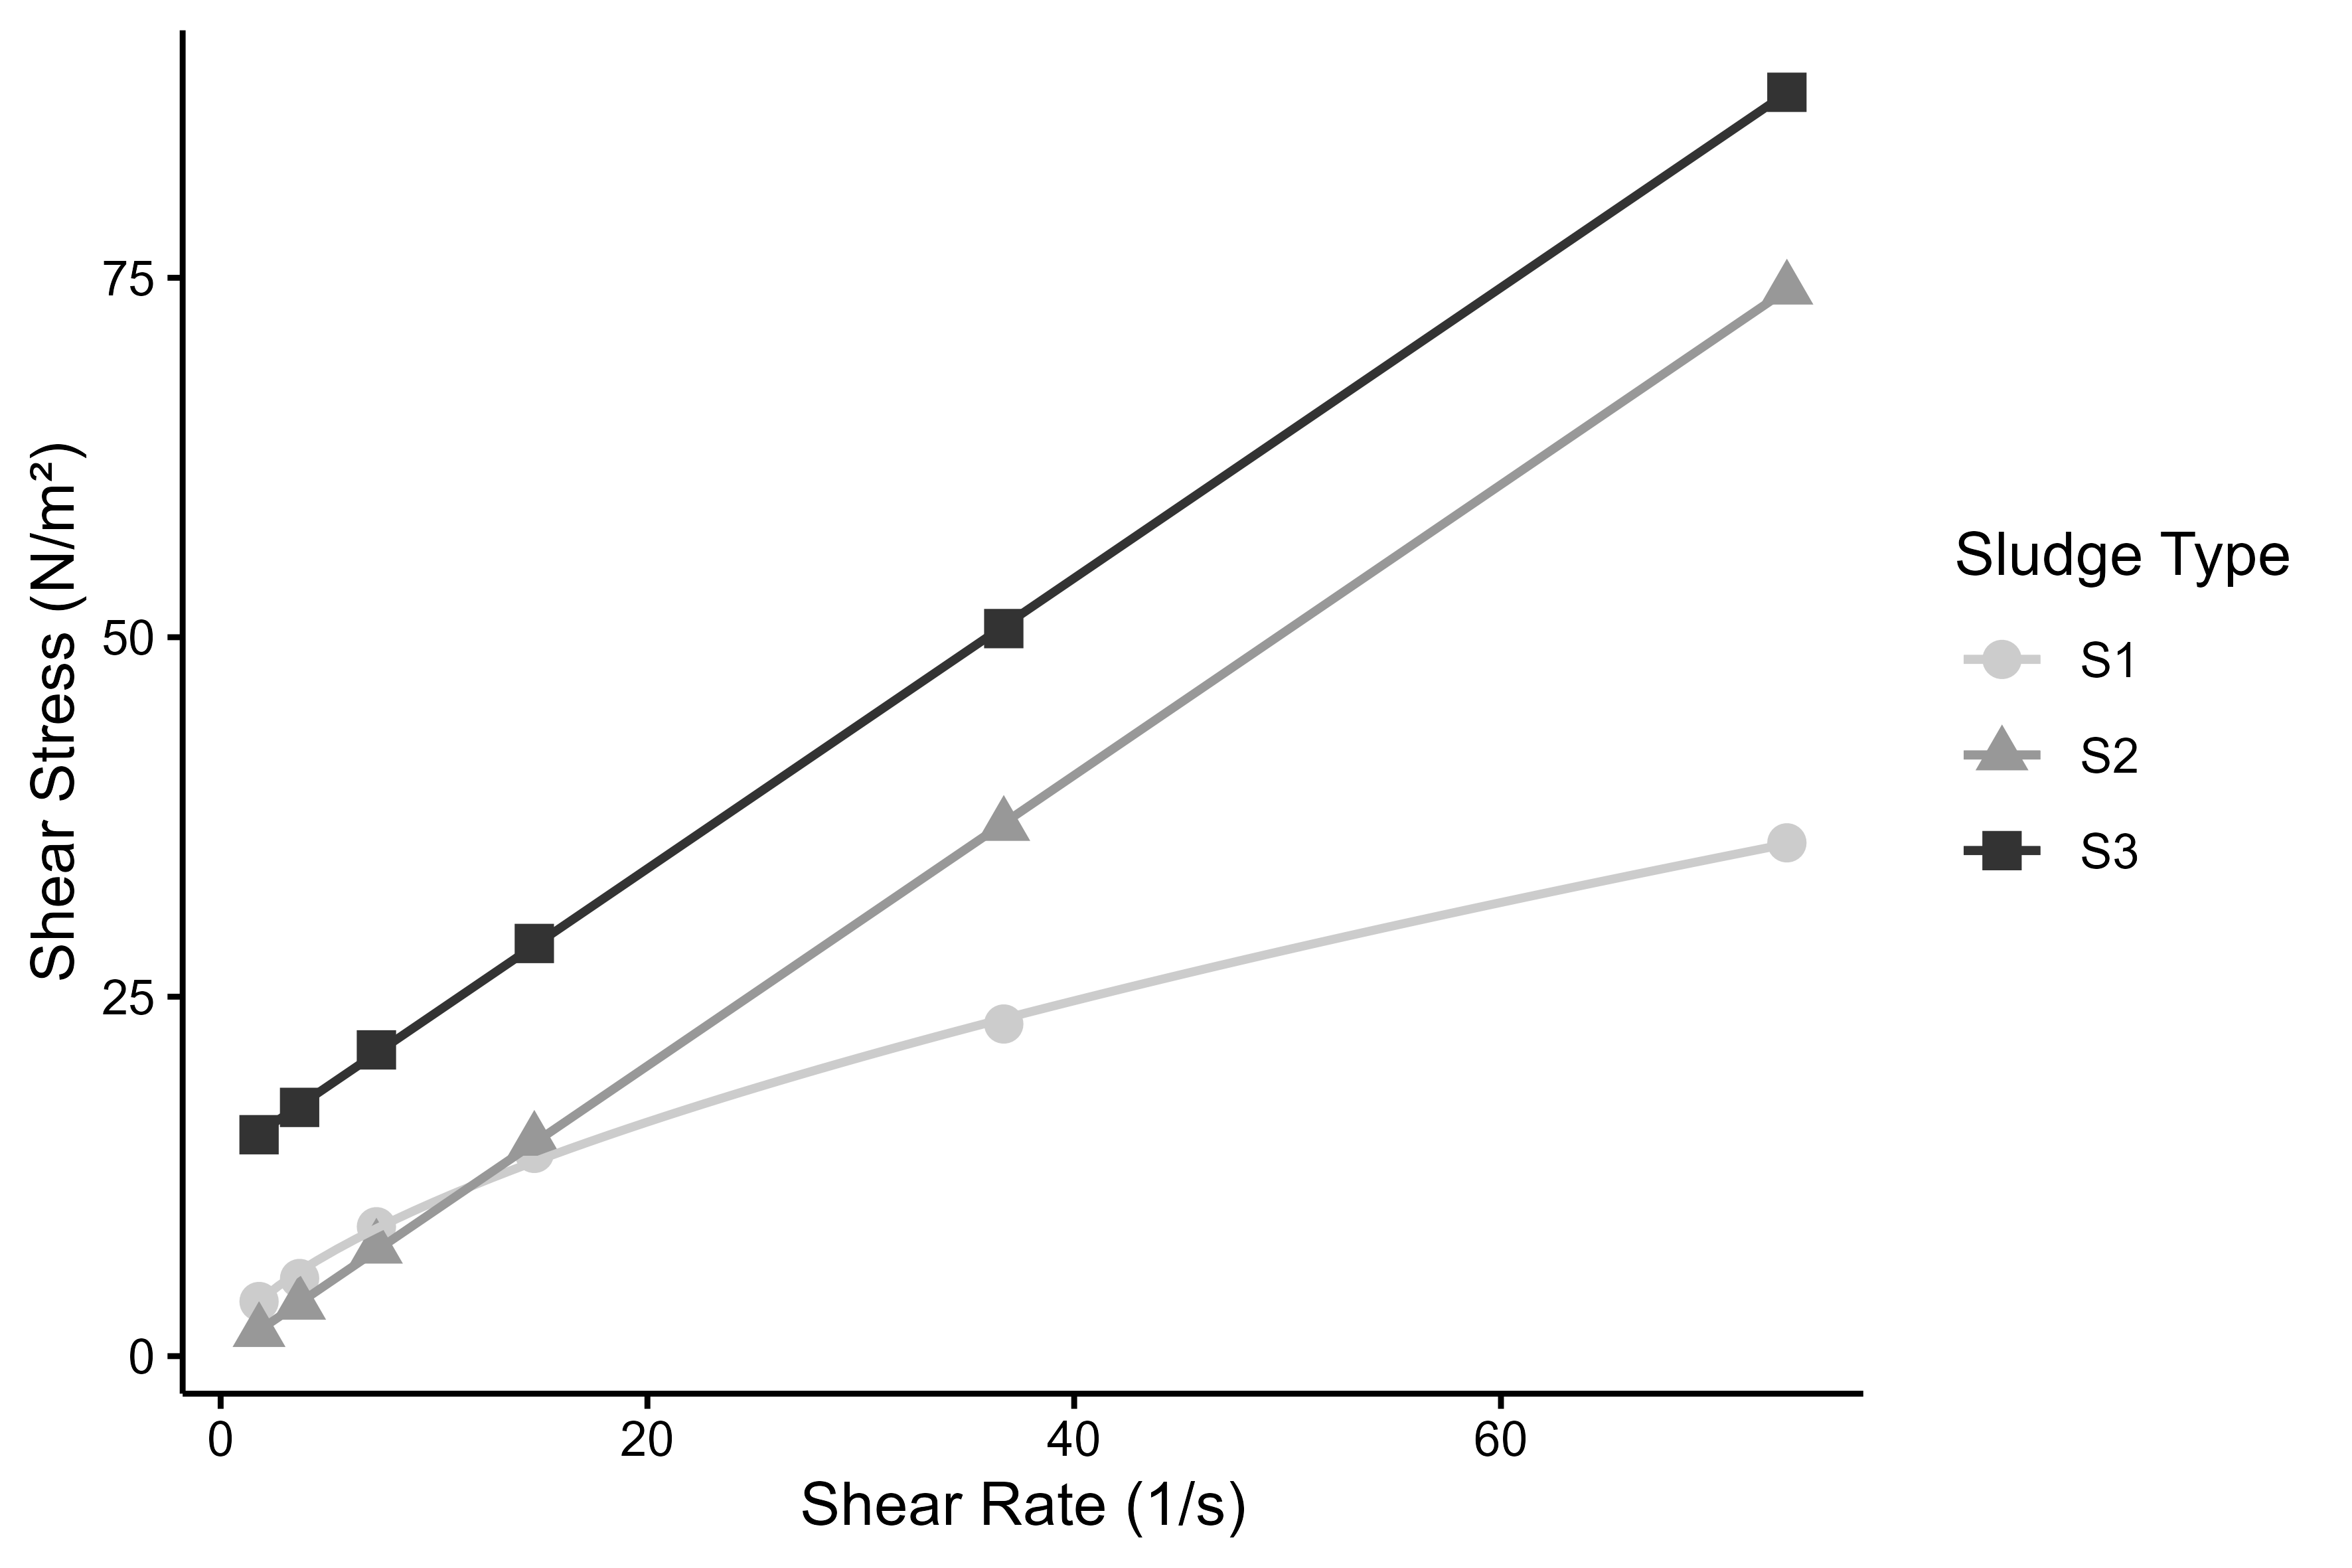
\includegraphics[scale=1]{homeworks/hw2/sludgeShear.png}
    \caption{Sludge rheology for three types of sludges}
    \label{fig:SludgeShear}
\end{figure}
The summarized version of the values for rheology models plotted with lines in Figure \ref{fig:SludgeShear} are given in Table \ref{tab:finalized}.
\begin{table}[ht]
    \centering
    \caption{The sludge analysis summary}
    \begin{tabular}{cccccc}
    \toprule
    \textbf{Sludge \#} & \textbf{Model Formula} & \textbf{Slope} & \textbf{Intercept} & \boldmath{$R^2$} & \textbf{Sludge Type} \\
    \midrule
    Sludge 1 & $\ln(y) = m\ln(x) + b$ & 0.61206 & 0.95382 & 0.9977 & \textsl{Pseudoplastic Fluid} \\
    Sludge 2 & $y = mx + b$ & 1.01075 & -0.02996 & 1.0000 & \textsl{Newtonian Fluid} \\
    Sludge 3 & $y = mx + b$ & 1.01035 & 13.69598 & 1.0000 & \textsl{Bingham Plastic Fluid} \\
    \bottomrule
    \end{tabular}
    \label{tab:finalized}
\end{table}
\section{}
\section*{Procedure}
\begin{minipage}[c]{0.6\textwidth}
Since there is no information on the flow rate for the raw sludge, \textbf{velocity}, \textbf{C}, \textbf{R}, and \textbf{S} in the SI Hazen–Williams formula (\ref{eq:H-W}) are missing. In this case, an empirically derived graph such as Figure 4.2 (pg. 120) in \textcite{sanin2011} can be used to determine the energy gradient for further estimations.\\
Since the sludge is different in terms of solids concentration, considering it is causing more head loss in the pipe, an altered C value should be used for any line while pumping sludge. Such modification can be applied for a tube with a C value of 100 \autocite{brisbin1957}.
\end{minipage}
\hfill
\begin{minipage}{0.35\textwidth}
\fbox{\parbox{0.95\textwidth}{\textbf{Assumptions}\\Solid concentration = 4\%\\Full pipe, pressurized flow\\No exit or minor losses\\Turbulent flow conditions\\No thixotropic behavior\\Not obstructed pipe\\Hazen–Williams Equation}}
\end{minipage}
\medskip
\begin{equation}
    v=0.85*C*R^{0.63}*S^{0.54} \label{eq:H-W}
\end{equation}
where:
\begin{itemize}[label = ]
    \item $v$ is the velocity (m/s),
    \item $C$ is the Hazen–Williams coefficient,
    \item $R$ is the hydraulic radius (m), and
    \item $S$ is the slope of the energy grade line (m/m).
\end{itemize}
\begin{table}[ht]
    \centering
    \caption{Hazen–Williams Coefficients for Various Solids Concentrations of Raw Sludge \autocite{brisbin1957}}
    \begin{tabular}{cc}
    \toprule
    Percent Total Solids & Apparent H-W Coefficient, Based on C = 100 for Water \\
    \midrule
    0 & 100 \\
    2 & 81 \\
    \textbf{4} & \textbf{61} \\
    6 & 45 \\
    8.5 & 32 \\
    10 & 25 \\
    \bottomrule
    \end{tabular}
    \label{tab:H-WCoeffs}
\end{table}
\section*{Calculations}
Assuming v = 1.22 m/s (4 ft/s) with 4\% solid concentration yields \autocite{sanin2011}:\\
$S = 0.04$\\
$S = h_L/L$\\
$h_L = 0.04*6000 = 240 \text{ m head-loss experienced.}$\\
\textbf{The total head required:}\\
$\text{Head} = h_L + \text{Static Head}$\\
$240 + 26 = \boxed{266 \text{ m}} \text{ Head required.}$\\
\textbf{The pipe diameter:}\\
Using Table \ref{tab:H-WCoeffs}, 4\% solid concentration results in C with the value of 61.\\
$1.22=0.85*61*(D/4)^{0.63}*0.04^{0.54}$\\
$D = 0.1643 \text{ m} \approx \boxed{165 \text{ mm}}$
\section*{Verification}
\begin{itemize}
    \item Velocity value checks for being in the turbulent region (> 0.9 m/s) \autocite{sanin2011, metcalf2014}.
    \item Diameter value is in the economically feasible range (150 - 200 mm) \autocite{sanin2011, vesilind1988, metcalf2014}.
    \item C value is taken from an experimental study that works with the other assumptions \autocite{brisbin1957}.
    \item Although the head-loss value is high, this is common in sludge pumping \autocite{sanin2011}. Since the assumption of 4\% solid content in the slurry affects this number dramatically, lower solid content cases for raw primary sludge would be less severe. Raw primary sludge solid content varies between 1 - 6 \% with a typical value of 3\% \autocite{metcalf2014}. Therefore, this estimation is on the safe side while being feasible.
\end{itemize}
\printbibliography
\end{document}